%%\documentclass[a4paper,12pt,oneside]{llncs}
\documentclass[12pt,letterpaper]{article}
\usepackage[right=2cm,left=3cm,top=2cm,bottom=2cm,headsep=0cm]{geometry}

%%%%%%%%%%%%%%%%%%%%%%%%%%%%%%%%%%%%%%%%%%%%%%%%%%%%%%%%%%%
%% Juego de caracteres usado en el archivo fuente: UTF-8
\usepackage{ucs}
\usepackage[utf8x]{inputenc}

%%%%%%%%%%%%%%%%%%%%%%%%%%%%%%%%%%%%%%%%%%%%%%%%%%%%%%%%%%%
%% Juego de caracteres usado en la salida dvi
%% Otra posibilidad: \usepackage{t1enc}
\usepackage[T1]{fontenc}

%%%%%%%%%%%%%%%%%%%%%%%%%%%%%%%%%%%%%%%%%%%%%%%%%%%%%%%%%%%
%% Ajusta maergenes para a4
%\usepackage{a4wide}

%%%%%%%%%%%%%%%%%%%%%%%%%%%%%%%%%%%%%%%%%%%%%%%%%%%%%%%%%%%
%% Uso fuente postscript times, para que los ps y pdf queden y pequeños...
\usepackage{times}

%%%%%%%%%%%%%%%%%%%%%%%%%%%%%%%%%%%%%%%%%%%%%%%%%%%%%%%%%%%
%% Posibilidad de hipertexto (especialmente en pdf)
%\usepackage{hyperref}
\usepackage[bookmarks = true, colorlinks=true, linkcolor = black, citecolor = black, menucolor = black, urlcolor = black]{hyperref}

%%%%%%%%%%%%%%%%%%%%%%%%%%%%%%%%%%%%%%%%%%%%%%%%%%%%%%%%%%%
%% Graficos 
\usepackage{graphics,graphicx}

%%%%%%%%%%%%%%%%%%%%%%%%%%%%%%%%%%%%%%%%%%%%%%%%%%%%%%%%%%%
%% Ciertos caracteres "raros"...
\usepackage{latexsym}

%%%%%%%%%%%%%%%%%%%%%%%%%%%%%%%%%%%%%%%%%%%%%%%%%%%%%%%%%%%
%% Matematicas aun más fuertes (american math dociety)
\usepackage{amsmath}

%%%%%%%%%%%%%%%%%%%%%%%%%%%%%%%%%%%%%%%%%%%%%%%%%%%%%%%%%%%
\usepackage{multirow} % para las tablas
\usepackage[spanish,es-tabla]{babel}

%%%%%%%%%%%%%%%%%%%%%%%%%%%%%%%%%%%%%%%%%%%%%%%%%%%%%%%%%%%
%% Fuentes matematicas lo mas compatibles posibles con postscript (times)
%% (Esto no funciona para todos los simbolos pero reduce mucho el tamaño del
%% pdf si hay muchas matamaticas....
\usepackage{mathptm}

%%% VARIOS:
%\usepackage{slashbox}
\usepackage{verbatim}
\usepackage{array}
\usepackage{listings}
\usepackage{multirow}

%% MARCA DE AGUA
%% Este package de "draft copy" NO funciona con pdflatex
%%\usepackage{draftcopy}
%% Este package de "draft copy" SI funciona con pdflatex
%%%\usepackage{pdfdraftcopy}
%%%%%%%%%%%%%%%%%%%%%%%%%%%%%%%%%%%%%%%%%%%%%%%%%%%%%%%%%%%
%% Indenteacion en español...
\usepackage[spanish]{babel}

\usepackage{listings}
% Para escribir código en C
% \begin{lstlisting}[language=C]
% #include <stdio.h>
% int main(int argc, char* argv[]) {
% puts("Hola mundo!");
% }
% \end{lstlisting}


\title{Análisis}
\author{Jesús Rodríguez Heras}

\begin{document}
	
	\maketitle
	\begin{abstract} %Poner esto en todas las prácticas de PCTR
		\begin{center}
			Análisis de resultados del ejercicio 3 de la práctica 7.
		\end{center}
	\end{abstract}
	\thispagestyle{empty}
	\newpage
	
%	\tableofcontents
%	\newpage
	
	%%\listoftables
	%%\newpage
	
	%%\listoffigures
	%%\newpage
	
	%%%% REAL WORK BEGINS HERE:
	
	%%Configuracion del paquete listings
	\lstset{language=bash, numbers=left, numberstyle=\tiny, numbersep=10pt, firstnumber=1, stepnumber=1, basicstyle=\small\ttfamily, tabsize=1, extendedchars=true, inputencoding=latin1}

%\section{Integral de la función $sen(x)$}
\begin{center}
	\begin{table}[htbp]
		\begin{center}
			\begin{tabular}{|c|c|c|c|}
				\hline
				\textbf{Puntos} & \textbf{intParalelauniCont} & \textbf{intParalelomultiCont} & \textbf{intParaleloFutureCont}  \\
				\hline 
				$10^6$ & 0.11 & 0.074 & 0.064 \\ \hline
				$5*10^6$ & 0.303 & 0.192 & 0.166 \\ \hline
				$10^7$ & 0.539 & 0.311 & 0.272 \\ \hline
				$5*10^7$ & 2.522 & 1.262 & 1.002 \\ \hline
				$10^8$ & 4.704 & 2.419 & 1.916 \\ \hline
				$5*10^8$ & 22.923 & 12.066 & 9.185 \\ \hline
				$10^9$ & 45.076 & 23.643 & 18.295 \\ \hline
			\end{tabular}
			\caption{Valores en segundos del tiempo usado por cada algoritmo.}
			\label{tabla:Valores en segundos del tiempo usado por cada algoritmo}
		\end{center}
	\end{table}
\end{center}
%\newpage
\begin{figure}[h]
	\begin{center}
		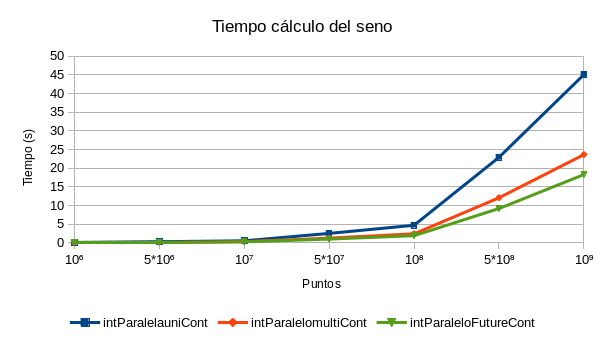
\includegraphics[scale=1]{TiempoSeno.png}
		\caption{Valores del tiempo del calculo de la integral de sen(x).}
		\label{fig:Valores del tiempo del calculo de la integral de sen(x)}
	\end{center}
\end{figure}
Tal y como se ve en la gráfica y en la tabla el algoritmo \texttt{intParaleloFutureCont.java} es un poco más eficiente que el algoritmo \texttt{intParalelomultiCont.java}. La diferencia empieza a notarse a partir de los 5 millones de puntos y, de ahí en adelante, dicha diferencia va creciendo poco a poco.



\end{document}